\chapter{Terbuat dari Apa Benda-Benda?}\label{ch:g1:materials-around-us}

Lihatlah meja sarapan. Ada sendok, segelas susu, garpu, serbet,
mangkuk, dan sebuah sweter yang tergantung di sandaran kursi. Banyak
sekali \omterm{def:g1:materials-around-us:object}{bendanya}, dan masing-masing terbuat dari sesuatu: sendoknya dari
kayu, garpunya dari logam, gelasnya dari kaca, serbetnya dari kertas,
mangkuknya dari plastik, sweternya dari wol. Satu meja penuh \omterm{def:g1:materials-around-us:object}{benda},
tetapi semuanya terbuat dari segelintir \omterm{def:g1:materials-around-us:material}{bahan} saja. Bab ini membahas
\omterm{def:g1:materials-around-us:material}{bahan-bahan} itu.

\begin{omfigure}
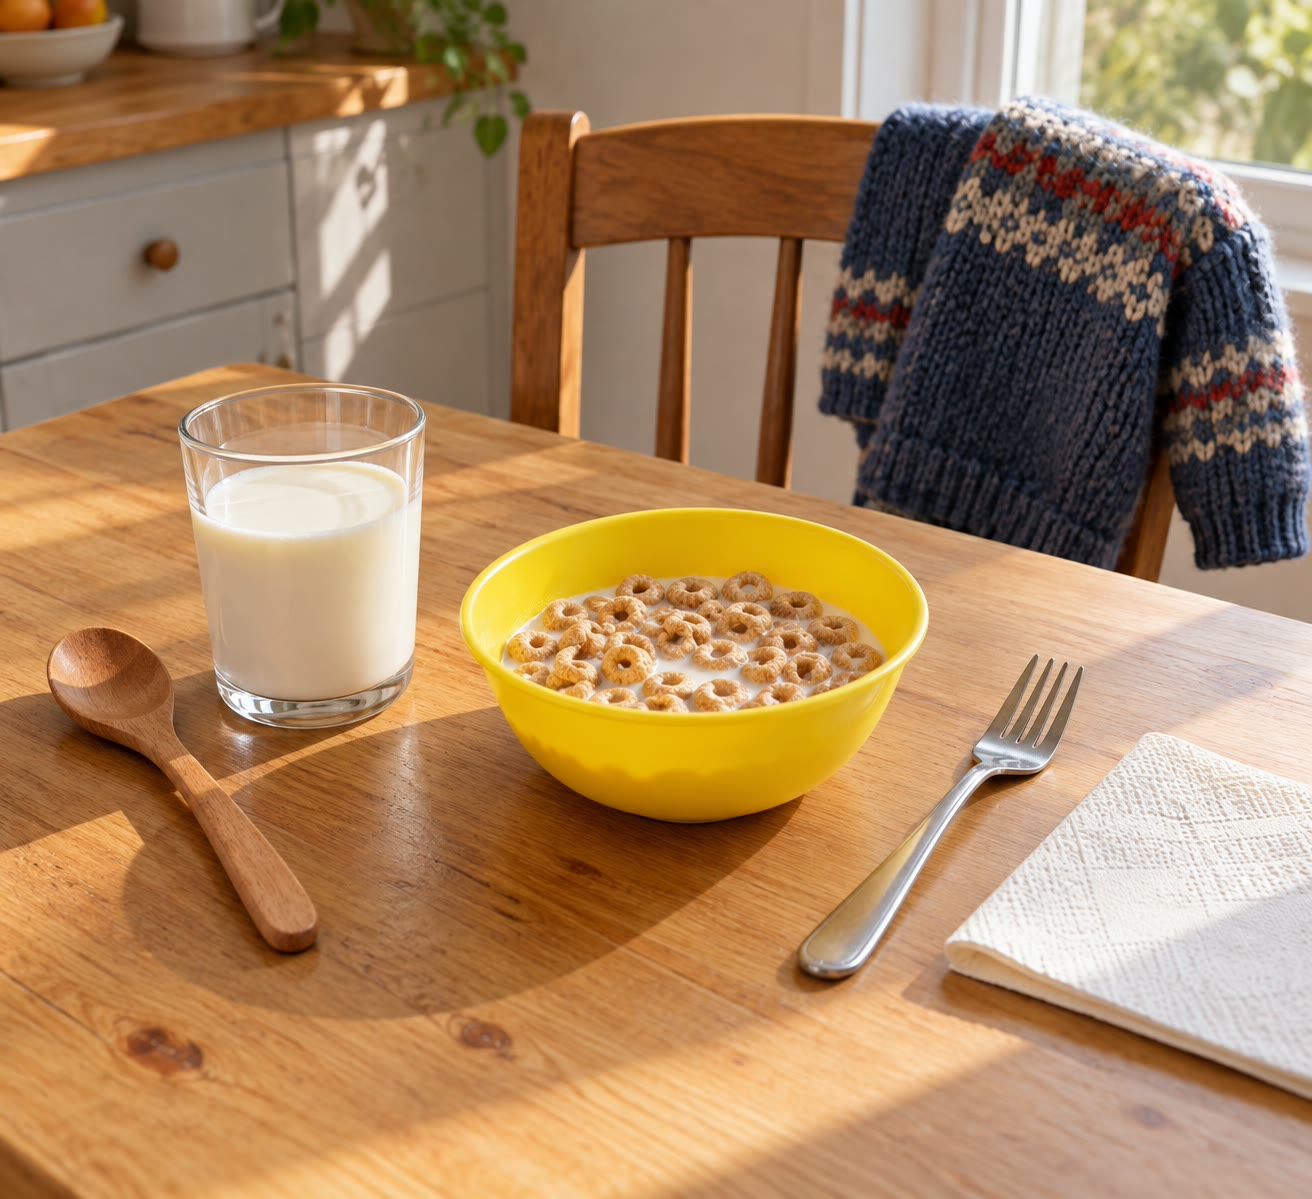
\includegraphics[width=0.62\linewidth]{images/book1/ai/g1-breakfast-table.jpg}

{\small Meja sarapan: banyak \omterm{def:g1:materials-around-us:object}{benda}, terbuat dari sedikit \omterm{def:g1:materials-around-us:material}{bahan}.}
\end{omfigure}

\section{Benda dan bahan}

\begin{definition}[Benda]\label{def:g1:materials-around-us:object}
Sebuah \emph{benda}\index{benda} adalah sesuatu yang dapat kita lihat
dan sentuh, dan sering dapat kita pegang dan pakai: sendok, kursi, bola,
jendela, sepatu.
\end{definition}

\begin{definition}[Bahan]\label{def:g1:materials-around-us:material}
Yang disebut \emph{bahan}\index{bahan} sebuah \omterm{def:g1:materials-around-us:object}{benda} adalah apa yang
membentuk \omterm{def:g1:materials-around-us:object}{benda} itu. Sendok dapat terbuat dari kayu, dari logam, atau
dari plastik: sendok adalah \omterm{def:g1:materials-around-us:object}{bendanya}, kayu adalah bahannya.
\end{definition}

\begin{example}[Satu benda, tiga bahan]\label{ex:g1:materials-around-us:spoons}
Tiga sendok terletak berjajar. Bentuknya sama dan kegunaannya sama,
jadi ketiganya \omterm{def:g1:materials-around-us:object}{benda} yang sejenis. Tetapi yang satu terbuat dari kayu,
yang satu dari logam, dan yang satu lagi dari plastik: tiga \omterm{def:g1:materials-around-us:material}{bahan} yang
berbeda.
\end{example}

\begin{omfigure}
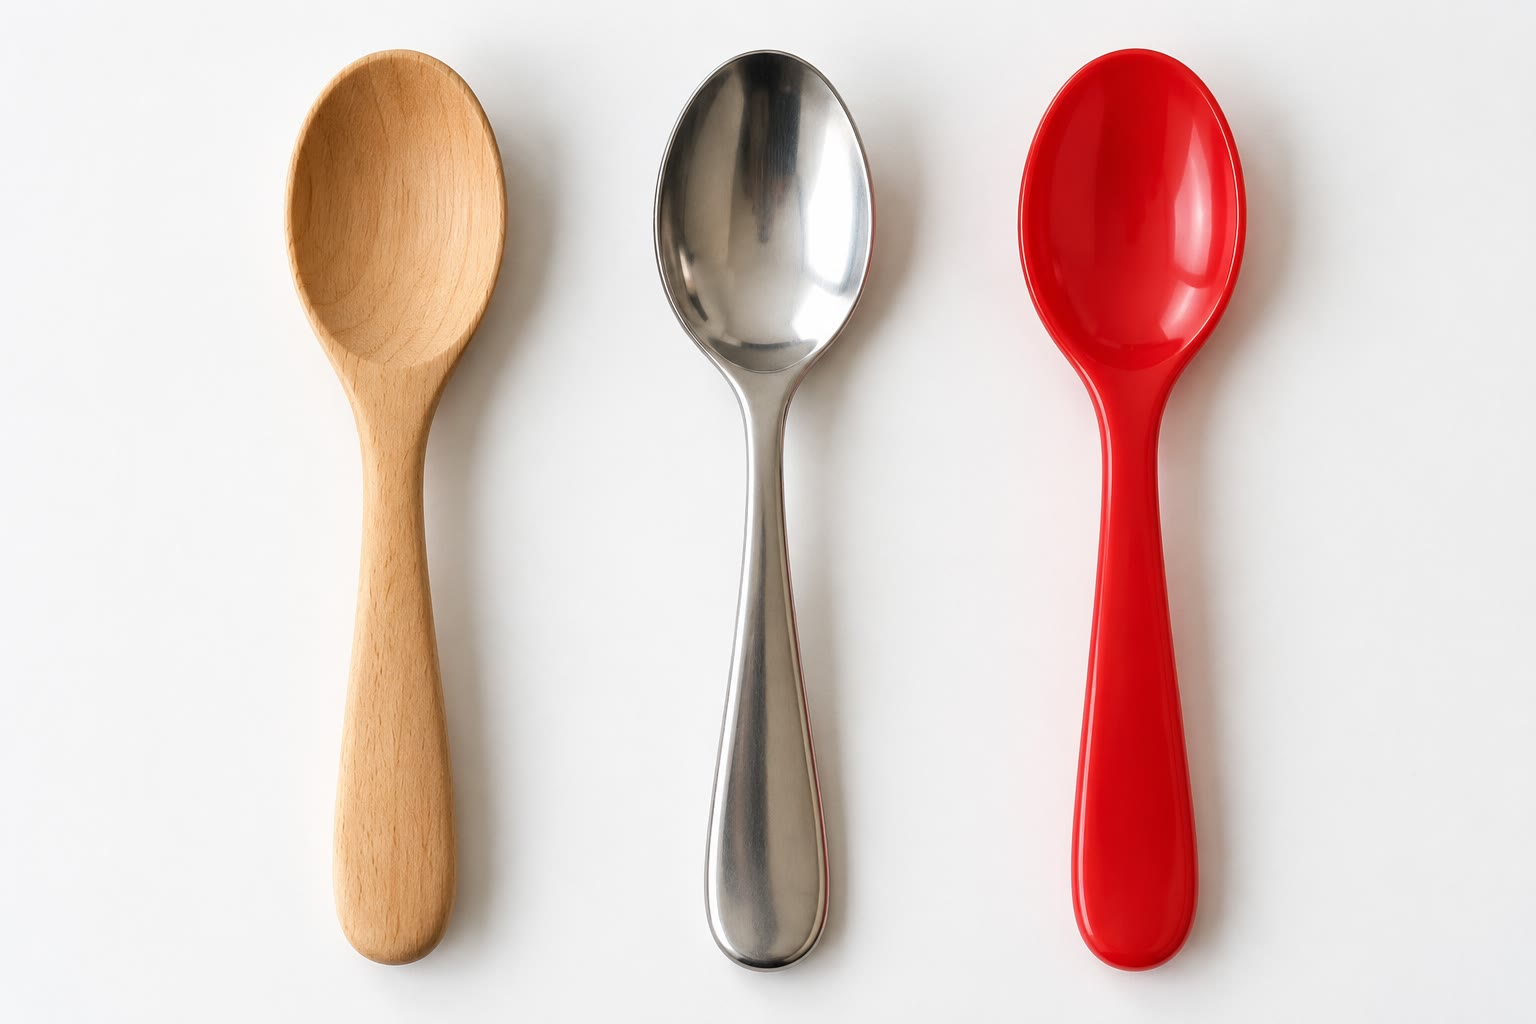
\includegraphics[width=0.55\linewidth]{images/book1/ai/g1-three-spoons.jpg}

{\small Tiga sendok: \omterm{def:g1:materials-around-us:object}{benda} yang sama, tiga \omterm{def:g1:materials-around-us:material}{bahan} --- kayu, logam, dan
plastik.}
\end{omfigure}

\begin{example}[Satu bahan, banyak benda]\label{ex:g1:materials-around-us:wood}
Kayu adalah \omterm{def:g1:materials-around-us:material}{bahan} sebuah pensil, kursi, pintu, kereta mainan, dan
sendok kayu. Banyak \omterm{def:g1:materials-around-us:object}{benda} yang berbeda dapat terbuat dari \omterm{def:g1:materials-around-us:material}{bahan} yang
sama.
\end{example}

\begin{remark}[Benda dari beberapa bahan]\label{rem:g1:materials-around-us:several}
Banyak \omterm{def:g1:materials-around-us:object}{benda} terbuat dari lebih dari satu \omterm{def:g1:materials-around-us:material}{bahan}. Gunting mempunyai
bilah dari logam dan pegangan dari plastik. Pensil bagian luarnya kayu
dan bagian dalamnya sebatang grafit kelabu. Jendela adalah kaca dalam
bingkai kayu, logam, atau plastik.
\end{remark}

\section{Tujuh bahan yang umum}

\begin{proposition}[Bahan di sekeliling kita]\label{prop:g1:materials-around-us:seven}
Sebagian besar \omterm{def:g1:materials-around-us:object}{benda} di sekitar kita terbuat dari beberapa \omterm{def:g1:materials-around-us:material}{bahan} yang
umum:
\begin{itemize}
  \item \textbf{kayu}: meja, kursi, pensil, pintu;
  \item \textbf{logam}: garpu, kunci, paku, panci, sepeda;
  \item \textbf{kaca}: jendela, stoples, botol, gelas;
  \item \textbf{plastik}: mangkuk, botol, mainan, ember;
  \item \textbf{kertas} dan karton: buku, serbet, kotak;
  \item \textbf{kain}: pakaian, gorden, tas --- dari wol, katun, atau
        benang lain;
  \item \textbf{batu}: dinding, anak tangga, kerikil, patung.
\end{itemize}
\end{proposition}

\begin{omfigure}
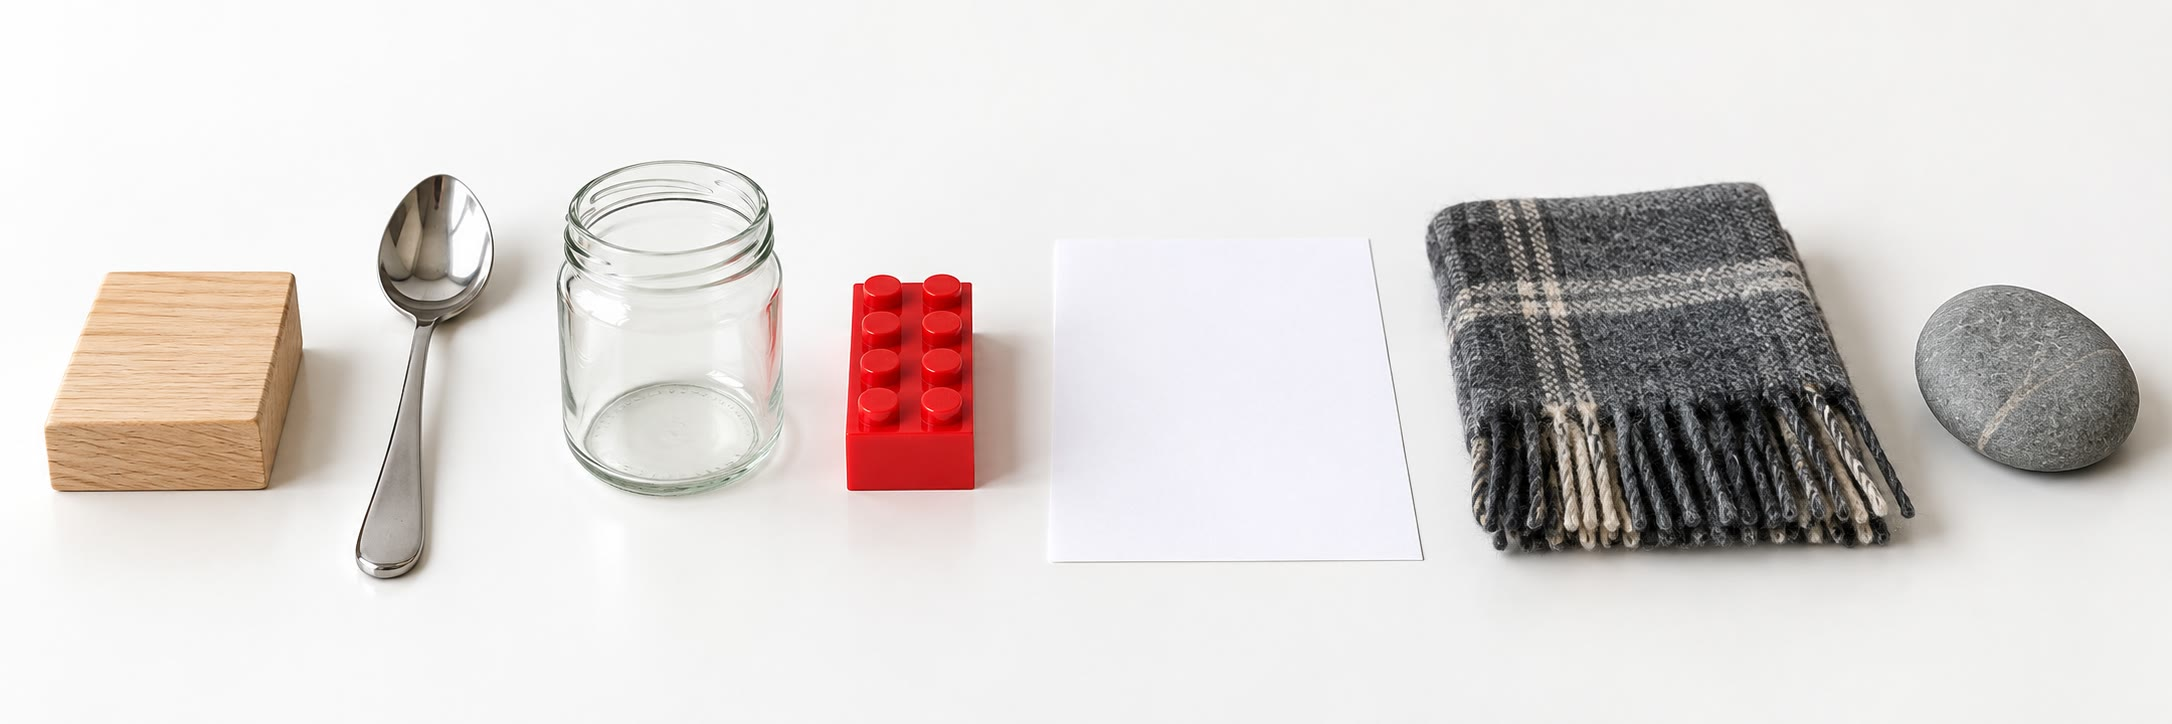
\includegraphics[width=0.75\linewidth]{images/book1/ai/g1-material-samples.jpg}

{\small Tujuh contoh \omterm{def:g1:materials-around-us:material}{bahan}, dari kiri ke kanan: kayu, logam, kaca,
plastik, kertas, kain (wol), dan batu.}
\end{omfigure}

\begin{remark}[Nama yang juga nama bahan]\label{rem:g1:materials-around-us:names}
Kaca jendela sering kita sebut ``kaca'' saja karena terbuat dari
kaca, dan selembar kertas cukup disebut ``kertas''. Nama
\omterm{def:g1:materials-around-us:object}{bendanya} dan nama \omterm{def:g1:materials-around-us:material}{bahannya} menjadi sama. Kalau kita berbicara tentang
\omterm{def:g1:materials-around-us:material}{bahan}, yang kita maksud adalah zatnya, bukan \omterm{def:g1:materials-around-us:object}{bendanya}.
\end{remark}

\section{Sifat-sifat bahan}

\begin{definition}[Sifat bahan]\label{def:g1:materials-around-us:property}
Yang disebut \emph{sifat bahan}\index{sifat bahan} adalah
sesuatu tentang \omterm{def:g1:materials-around-us:material}{bahan} itu yang dapat kita ketahui dengan melihat,
meraba, atau mengujinya: apakah \omterm{def:g1:materials-around-us:material}{bahan} itu keras atau lunak? Dapatkah
kita melihat menembusnya? Apakah magnet menariknya? Apakah ia
terapung di air atau tenggelam?
\end{definition}

\begin{example}[Keras dan lunak]\label{ex:g1:materials-around-us:hard}
Kerikil itu keras: kalau ditekan dengan ibu jari, tidak ada bekasnya.
Syal wol itu lunak: ia mudah melengkung dan terlipat di tangan. Kayu,
logam, kaca, dan batu keras; kain dan kertas lunak dan mudah
dilipat.
\end{example}

\begin{example}[Tembus pandang]\label{ex:g1:materials-around-us:see-through}
Kita dapat melihat kebun lewat jendela: kaca meneruskan cahaya, dan kita
katakan kaca itu \emph{bening}. Kita tidak dapat melihat menembus pintu
kayu, dinding bata, atau panci logam. Sebagian plastik bening, seperti
botol air minum; sebagian lagi tidak, seperti balok mainan merah.
\end{example}

\begin{example}[Ditarik magnet]\label{ex:g1:materials-around-us:magnet}
Magnet menarik penjepit kertas dari baja, paku baja, atau kunci besi ke
arahnya. Magnet tidak menarik kayu, kaca, plastik, kertas, kain, atau
batu. Anehnya, magnet juga tidak menarik semua logam: kaleng minuman
dari aluminium dan kawat tembaga tetap di tempatnya. Magnet menarik
\omterm{def:g1:materials-around-us:object}{benda} dari besi dan dari baja, yang sebagian besar terdiri atas besi.
\end{example}

\begin{omfigure}
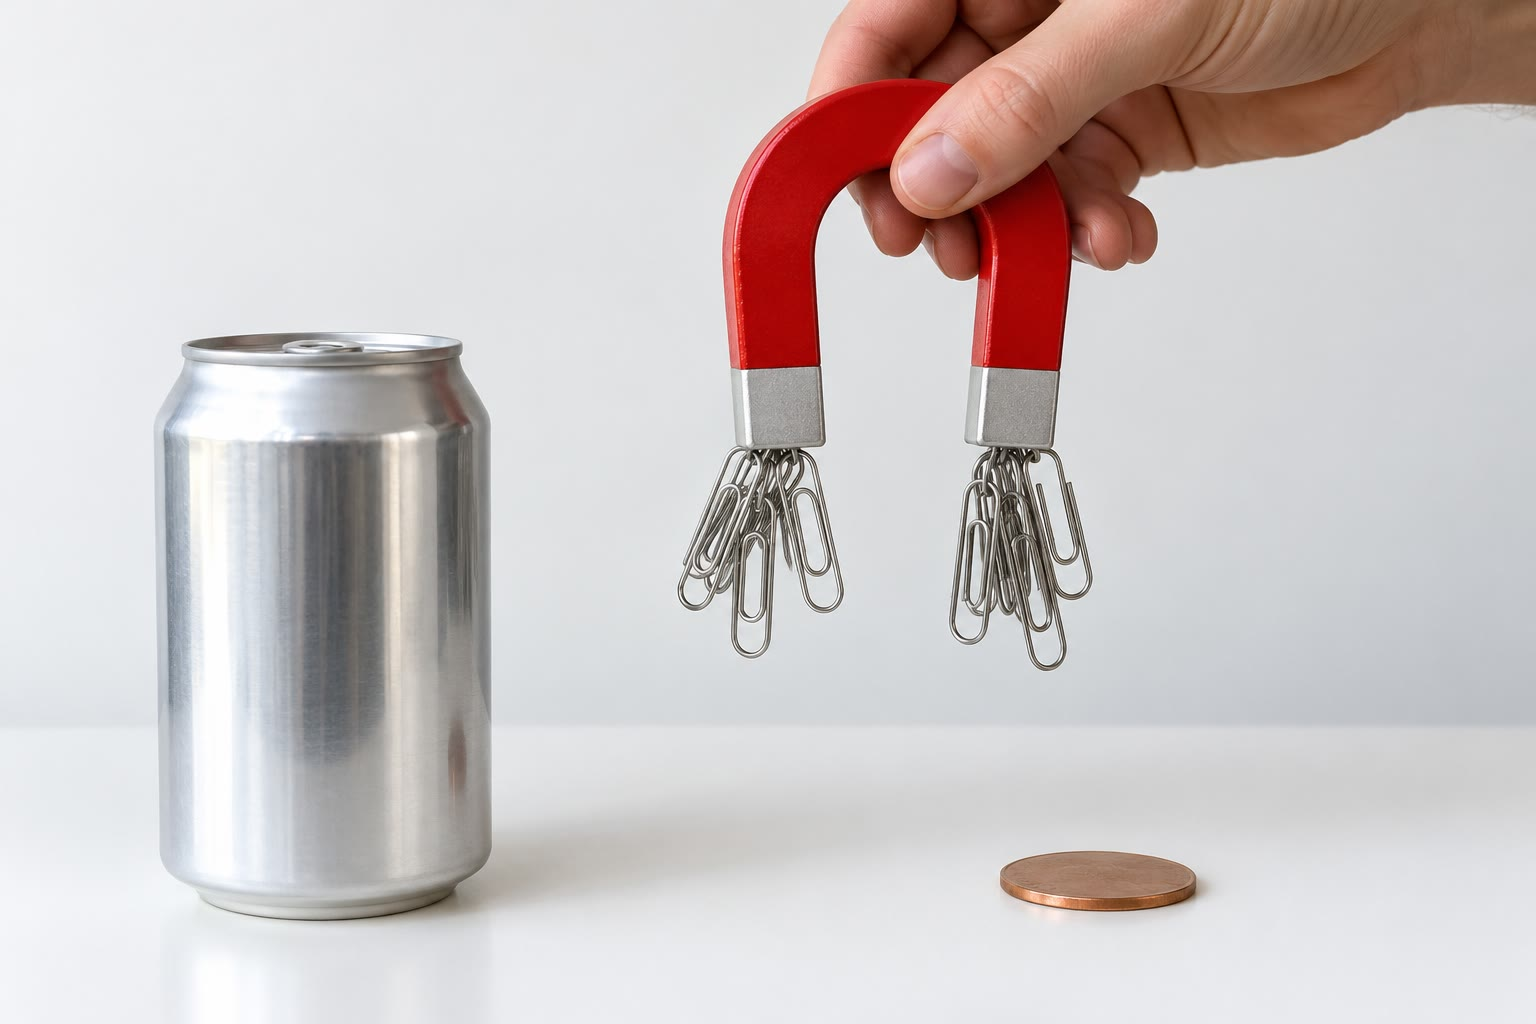
\includegraphics[width=0.55\linewidth]{images/book1/ai/g1-magnet-clips.jpg}

{\small Magnet mengangkat penjepit kertas dari baja. Kaleng aluminium
dan cakram tembaga di atas meja tetap di tempatnya.}
\end{omfigure}

\begin{example}[Terapung dan tenggelam]\label{ex:g1:materials-around-us:float}
Masukkan beberapa \omterm{def:g1:materials-around-us:object}{benda} ke dalam baskom berisi air. Balok kayu dan
tutup botol plastik terapung. Kerikil, kelereng kaca, dan paku baja
tenggelam ke dasar. Terapung atau tenggelamnya suatu \omterm{def:g1:materials-around-us:object}{benda} juga
merupakan \omterm{def:g1:materials-around-us:property}{sifat bahannya}.
\end{example}

\begin{omfigure}
\begin{tikzpicture}[font=\small]
  % the basin
  \fill[omWater!80] (0,0) rectangle (9,2.2);
  \draw[omGlass, line width=0.8pt] (-0.1,2.7) -- (0,2.6) -- (0,0) -- (9,0)
    -- (9,2.6) -- (9.1,2.7);
  % floating: wooden block, plastic cap
  \fill[brown!55, draw=brown!70!black] (0.8,2.0) rectangle (2.2,2.5);
  \fill[red!70, draw=red!50!black] (3.7,2.05) rectangle (4.3,2.35);
  % sunk: pebble, marble, nail
  \fill[black!35, draw=black!60] (5.0,0.25) ellipse (0.45 and 0.22);
  \shade[ball color=cyan!40] (6.5,0.2) circle (0.18);
  \fill[black!55] (7.6,0.06) rectangle (8.6,0.14);
  \fill[black!55] (7.52,0.02) rectangle (7.62,0.18);
  % labels
  \node[anchor=south] at (1.5,2.75) {balok kayu};
  \node[anchor=south] at (4.0,2.75) {tutup plastik};
  \node[anchor=north] at (5.0,-0.1) {kerikil};
  \node[anchor=north] at (6.5,-0.1) {kelereng};
  \node[anchor=north] at (8.1,-0.1) {paku};
  \node[anchor=west, align=left] at (9.3,2.2) {yang ini terapung};
  \node[anchor=west, align=left] at (9.3,0.2) {yang ini tenggelam};
\end{tikzpicture}

{\small Di dalam baskom berisi air: balok kayu dan tutup plastik
terapung; kerikil, kelereng kaca, dan paku baja tenggelam.}
\end{omfigure}

\section{Mengelompokkan bahan}

\begin{method}[Mengelompokkan menurut satu sifat]\label{met:g1:materials-around-us:sort}
Untuk mengelompokkan setumpuk \omterm{def:g1:materials-around-us:object}{benda}:
\begin{enumerate}
  \item pilihlah \textbf{satu} pertanyaan, misalnya ``Apakah magnet
        menariknya?'';
  \item ujilah setiap \omterm{def:g1:materials-around-us:object}{benda} dan masukkan ke kelompok ``ya'' atau ke
        kelompok ``tidak'';
  \item lalu, kalau kamu mau, kelompokkan lagi setiap kelompok dengan
        pertanyaan lain.
\end{enumerate}
Satu pertanyaan sekali jalan: dengan begitu setiap \omterm{def:g1:materials-around-us:object}{benda} mendapat tepat
satu tempat.
\end{method}

\begin{omfigure}
\begin{tikzpicture}[font=\small]
  \draw[omDef, line width=1pt] (0,0) circle (2.3);
  \draw[omProp, line width=1pt] (2.4,0) circle (2.3);
  \node[omDef, font=\small\bfseries] at (-0.6,2.65) {terbuat dari logam};
  \node[omProp, font=\small\bfseries] at (3.0,2.65) {ditarik magnet};
  \node[font=\footnotesize, align=center] at (-1.1,0.35) {kaleng\\ minuman};
  \node[font=\footnotesize] at (-1.1,-0.35) {kawat tembaga};
  \node[font=\footnotesize] at (1.2,0.6) {paku baja};
  \node[font=\footnotesize] at (1.2,0) {kunci besi};
  \node[font=\footnotesize, align=center] at (1.2,-0.6) {penjepit\\ kertas};
  \node[font=\footnotesize] at (3.5,0) {(kosong)};
  \node[anchor=west] at (5.2,0.9) {sendok kayu};
  \node[anchor=west] at (5.2,0.3) {kelereng kaca};
  \node[anchor=west] at (5.2,-0.3) {syal wol};
  \node[anchor=west] at (5.2,-0.9) {kerikil};
\end{tikzpicture}

{\small Dua pertanyaan, dua lingkaran. Di dalam lingkaran biru: \omterm{def:g1:materials-around-us:object}{benda}
yang terbuat dari logam. Di dalam lingkaran jingga: \omterm{def:g1:materials-around-us:object}{benda} yang ditarik
magnet. Di dalam kedua lingkaran: \omterm{def:g1:materials-around-us:object}{benda} dari besi atau baja. Di luar
keduanya: semua \omterm{def:g1:materials-around-us:object}{benda} lainnya.}
\end{omfigure}

\begin{center}
\small
\begin{tabular}{lccc}
\hline
\omterm{def:g1:materials-around-us:object}{benda} (\omterm{def:g1:materials-around-us:material}{bahan}) & keras? & tembus pandang? & ditarik magnet? \\
\hline
balok (kayu) & ya & tidak & tidak \\
paku (baja) & ya & tidak & ya \\
kelereng (kaca) & ya & ya & tidak \\
tutup botol (plastik) & ya & tidak & tidak \\
lembaran (kertas) & tidak & tidak & tidak \\
syal (wol) & tidak & tidak & tidak \\
kerikil (batu) & ya & tidak & tidak \\
\hline
\end{tabular}
\end{center}

\section{Bahan yang tepat untuk tugasnya}

\begin{proposition}[Setiap bahan dipilih karena sifatnya]\label{prop:g1:materials-around-us:choose}
Orang memilih \omterm{def:g1:materials-around-us:material}{bahan} sebuah \omterm{def:g1:materials-around-us:object}{benda} sesuai dengan apa yang harus
dikerjakan \omterm{def:g1:materials-around-us:object}{benda} itu:
\begin{itemize}
  \item jendela harus memasukkan cahaya: jendela dibuat dari kaca, yang
        bening;
  \item jas hujan harus menahan hujan dan dapat dilipat: jas hujan
        dibuat dari plastik atau dari kain yang tidak dapat ditembus
        air;
  \item panci tidak boleh meleleh di atas kompor: panci dibuat dari
        logam;
  \item gagang panci tidak boleh membakar tangan: gagang itu sering
        dibuat dari kayu atau plastik keras, yang tidak sepanas logam;
  \item bantal harus empuk: bantal dibuat dari kain yang diisi bulu
        atau serat.
\end{itemize}
\end{proposition}

\begin{example}[Sebuah perahu]\label{ex:g1:materials-around-us:boat}
Perahu mainan harus terapung. Perahu itu dapat dibuat dari kayu atau
dari plastik. Perahu dari sebongkah batu pejal akan langsung tenggelam.
\end{example}

\begin{remark}[Kaca pecah]\label{rem:g1:materials-around-us:glass}
Kaca itu keras, tetapi dapat pecah, dan pecahannya tajam. Kalau ada
gelas yang pecah, orang dewasalah yang memungut pecahannya.
\end{remark}

\section{Latihan}

\begin{exercise}[$\star$]\label{exo:g1:materials-around-us:1}
Kursi itu \omterm{def:g1:materials-around-us:object}{benda} atau \omterm{def:g1:materials-around-us:material}{bahan}? Kayu itu \omterm{def:g1:materials-around-us:object}{benda} atau \omterm{def:g1:materials-around-us:material}{bahan}?
\end{exercise}

\begin{exercise}[$\star$]\label{exo:g1:materials-around-us:2}
Sebutkan \omterm{def:g1:materials-around-us:material}{bahan} setiap \omterm{def:g1:materials-around-us:object}{benda} berikut: kaca jendela, paku, kerikil,
buku, kaus kaki.
\end{exercise}

\begin{exercise}[$\star$]\label{exo:g1:materials-around-us:3}
Sebutkan dua \omterm{def:g1:materials-around-us:object}{benda} dari kayu dan dua \omterm{def:g1:materials-around-us:object}{benda} dari plastik.
\end{exercise}

\begin{exercise}[$\star$]\label{exo:g1:materials-around-us:4}
Carilah yang berbeda sendiri, dan katakan mengapa: sendok kayu, garpu
logam, sendok plastik, kursi kayu. (Perhatikan \omterm{def:g1:materials-around-us:material}{bahannya}.)
\end{exercise}

\begin{exercise}[$\star$]\label{exo:g1:materials-around-us:5}
\omterm{def:g1:materials-around-us:material}{Bahan} mana yang tembus pandang: kayu, kaca, atau batu?
\end{exercise}

\begin{exercise}[$\star$]\label{exo:g1:materials-around-us:6}
Sebuah magnet didekatkan ke paku baja, kelereng kaca, dan balok kayu.
\omterm{def:g1:materials-around-us:object}{Benda} mana yang ditariknya?
\end{exercise}

\begin{exercise}[$\star$]\label{exo:g1:materials-around-us:7}
Lihatlah gambar baskom. Berapa \omterm{def:g1:materials-around-us:object}{benda} yang terapung? Berapa yang
tenggelam?
\end{exercise}

\begin{exercise}[$\star$]\label{exo:g1:materials-around-us:8}
Gunting mempunyai bilah dan pegangan. Terbuat dari \omterm{def:g1:materials-around-us:material}{bahan} apa setiap
bagiannya? Apakah gunting terbuat dari satu \omterm{def:g1:materials-around-us:material}{bahan} atau dua?
\end{exercise}

\begin{exercise}[$\star$]\label{exo:g1:materials-around-us:9}
Lihatlah gambar dua lingkaran. Di lingkaran mana kaleng minuman berada?
Mengapa kaleng itu tidak berada di lingkaran jingga?
\end{exercise}

\begin{exercise}[$\star\star$]\label{exo:g1:materials-around-us:10}
Mengapa jendela dibuat dari kaca, bukan dari kayu?
\end{exercise}

\begin{exercise}[$\star\star$]\label{exo:g1:materials-around-us:11}
Sam ingin mengelompokkan 8 \omterm{def:g1:materials-around-us:object}{benda} ini dengan pertanyaan ``Apakah
magnet menariknya?'': paku baja, penjepit kertas, kerikil, sendok
kayu, kunci besi, kaleng minuman, kelereng kaca, dan kaus kaki wol.
Berapa \omterm{def:g1:materials-around-us:object}{benda} yang
masuk kelompok ``ya''? Berapa yang masuk kelompok ``tidak''?
\end{exercise}
